As explained in the previous chapter, we've created classes to represent some features related to blockchains. Thus, we can instantiate miners, blocks, block headers and blockchains.

\section{Sequential code}

Then, the first version of the code is about making these objects to work together. This is a sequential version where, in the end, we have one miner able to create blocks, mine them and build his blockchain.

When the job is done, we display the state of the blockchain: \newline

\begin{figure}[ht]
\centering
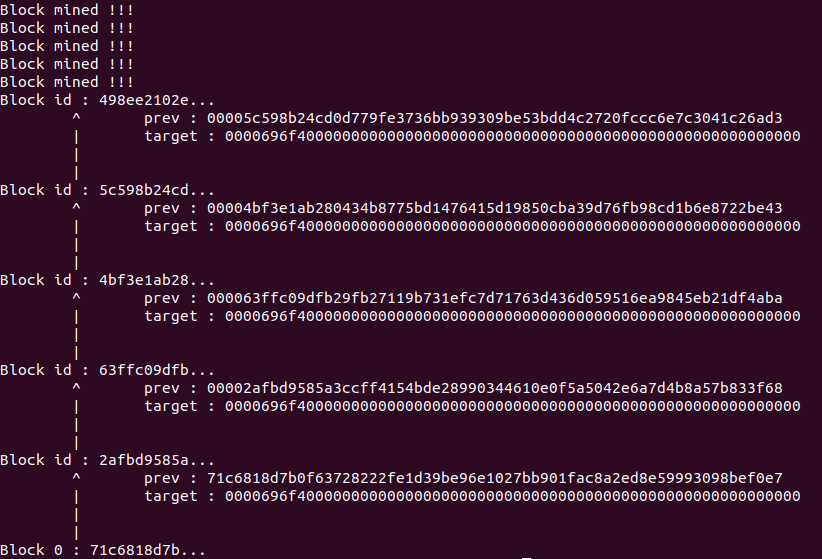
\includegraphics[width=10cm]{Figures/sequentialCode}
\caption{Example of execution}
\end{figure}
\medskip

We don't concentrate further in the analysis because the objective is to parallelize this code.

\section{Parallel code}

\paragraph{Transactions management}

As we mentioned, transaction management is simplified. So we decide to generate transactions with our specific generator and to communicate these transactions to all the miners. \newline

Thus, the first challenge is to generate and broadcast transactions. We arbitrary choose the miner 0 to generate the transactions, then he will serialize and broadcast them to the other miners.

At the same time, we manage the reception of these transactions by the others miners. They deserialize them and push them to their mempool. \newline

\paragraph{Communication through the network}

The most important challenge is to make the miners communicate about blocks they discovered. To do so, we created the following algorithm:

\clearpage

\begin{algorithm}
  \caption{Communication between miners}
  \begin{algorithmic}

    \WHILE{the mempool isn't empty}
      \STATE We fill a new block with transactions from the mempool

      \WHILE{No message received \&\& no block mined}
        \STATE We try to mine the block

        \IF{Block mined}
          \STATE We write related information into a log file
          \STATE We broadcast the block mined
        \ENDIF

        \STATE We check for messages

        \IF{Block received}
          \STATE Block reception algorithm (see below)
        \ELSIF{Blockchain received}
          \STATE We add the blockchain to ours
          \STATE We sort our chains to work on the longest
        \ELSIF{Blockchain request received}
          \STATE We send back the requested blockchain
        \ENDIF

      \ENDWHILE
    \ENDWHILE
  \end{algorithmic}
\end{algorithm}

\begin{algorithm}
  \caption{Block reception}

  \begin{algorithmic}
    \FOR{All our blockchains}
      \IF{The new block is the next one}
        \STATE We add it at the end
      \ELSIF{The new block is the last one}
        \STATE We do nothing
      \ELSE
        \FOR{All blocks in the chain}
          \IF{The new block and the current one are the same}
            \STATE We sent back this chain
          \ELSIF {The new block is the next of the current one}
            \STATE We create a forked chain including the new block
            \STATE We sort our chains
            \STATE We send our version of the chain
          \ENDIF
        \ENDFOR
      \ENDIF
    \ENDFOR

  \end{algorithmic}

\end{algorithm}

\subsection{Extra features}

\paragraph{Tests}

It's important to regularly test our code, especially to check if the communications are complete because this kind of error is quite hard to detect. There are some dedicated libraries to test our code but, in our case, we used a direct way by implementing controls to test our functions and print the results so we can check the correctness of our system. \newline

We can test sending and receiving a block, a blockchain or an empty blockchain. This increases our confidence in the code robustness.

\paragraph{Frequency estimation}

We've seen that the computational power of a miner is important because the higher his computational power the faster it will mine. Then, we created a code to estimate the frequency of a miner. \newline

To estimate the frequency, we use the instruction RDTSC (ReaD Time Stamp Counter) which reads the value of the register TSC. This register counts the number of cycles since the last reset. So we use the following algorithm to compute the number of cycles in 1 second: \newline

\begin{algorithm}
  \caption{Frequency estimation}

  \begin{algorithmic}
    \STATE int nbCycle = rdtsc()
    \STATE Wait for 1 second
    \STATE frequency = rdtsc() - nbCycle
  \end{algorithmic}
\end{algorithm}
\medskip

\paragraph{Logs}

All along the code, we write information in the log files to help analyze the blockchain at the end. For example: \newline

\begin{itemize}
  \item {[freq]} 2.4225  $\rightarrow$ Indicates the miner computational power in GHz.
  \item {[Tue Jul 23 17:40:48 2019]} 3fd2146979 26027 $\rightarrow$ Indicates the miner has mined a block with the exact time, the block ID and the duration in milliseconds.
  \item {[nbChains]} 1 $\rightarrow$ Indicates the number of forked chains the miner has made.
  \item {[i]} 47a9270fb6 $\rightarrow$ Indicates the beginning of the ith chain and its first block.
\end{itemize}
\medskip

\begin{figure}[ht]
\centering
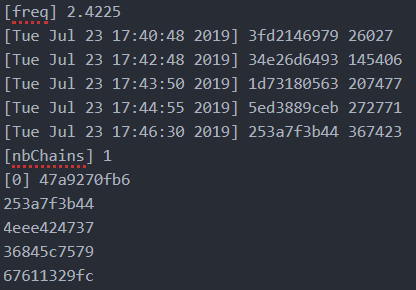
\includegraphics[width=8cm]{Figures/logExample}
\caption{Example of a log file}
\end{figure}
\medskip

We also write a general log file with the following data: \newline

\begin{itemize}
  \item {[nbTransactions]} 1000 $\rightarrow$ Indicates the number of transactions.
  \item {[nbProc]} 20 $\rightarrow$ Indicates the number of miners.
  \item {[difficulty]} 3 $\rightarrow$ Indicates the difficulty for the target (i.e. the number of zeros required at the beginning of the hash).
  \item {[finalTime]} 389194 $\rightarrow$ Indicates how long it took to complete the execution in milliseconds.
\end{itemize}



\section{Results}

\paragraph{Reading the logs}


\begin{enumerate}
  \item We read the file with the general data: nbProc, nbTransactions, difficulty.
  \item We read the file of each miner to get his frequency, the block mined and the blockchains.
  \item From the longest chain, we determine which miner has won a reward.
  \item We extract the data to display the timeline of the longest blockchain.
  \item We extract the times where the blocks were mined to compute statistics.
\end{enumerate}
\medskip

In the end, we display a table summing up the rewards and the forks of each miner, another table with statistics about the time needed to mine blocks and a timeline of the blockchain 10 blocks by 10 blocks. \newline

The following results were produced on the Geneva University cluster with a target starting with 5 zeros.

\paragraph{Analysis of the rewards and forks table}

This table is interesting in two points: \newline

\begin{enumerate}
  \item To analyze if the frequency and the number of rewards are correlated. The more a miner has computational power, the faster it should mine. \newline

  In our case, all miners have the same frequency because they were all located on the same node of the cluster.

  \item To observe the number of forks because this number is directly linked to the number of messages. If the number of forks is low, it means the consensus was obtained straight forward. On the other hand, if this number is high, it means the miners exchanged a lot of messages and probably wasted time on mining blocks which were finally not in the longest chain. \newline

  In our case, we see the number of forks is 1 for all miners so it means that our algorithm is efficient.
\end{enumerate}

\begin{figure}[ht]
\centering
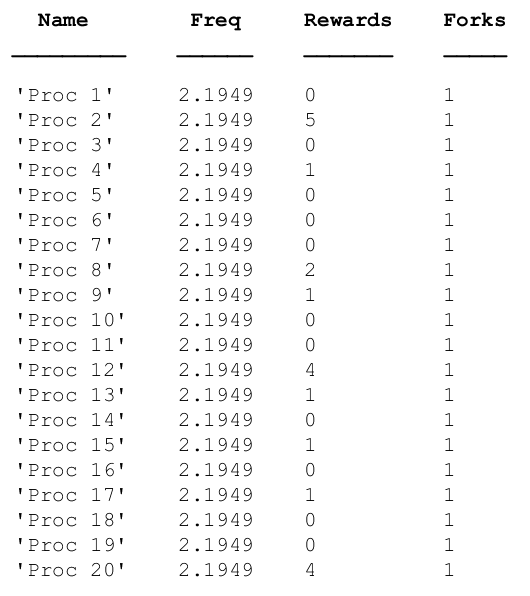
\includegraphics[width=10cm]{Figures/rewards}
\caption{Rewards won by the miners}
\end{figure}
\medskip

\paragraph{Analysis of the statistics table}

We can observe that the range is quite wide, from $\approx$ 9 minutes to 7 seconds, it means that some miners mined a block very quickly whereas some others took more time. This is because we choose the nonce in a uniform distribution so it's completely possible to obtain a right nonce after a few tries only. \newline

We can also note that the average time to mine a block is around 1 minute and 48 seconds, it's an arbitrary choice compared to the 10 minutes for the original blockchain.
\clearpage

\begin{figure}[ht]
\centering
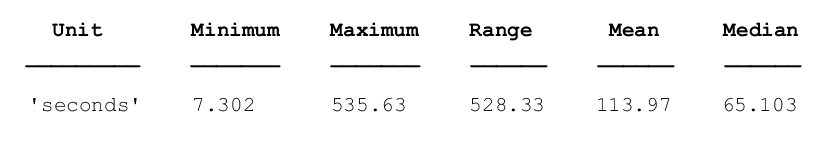
\includegraphics[width=10cm]{Figures/stats}
\caption{Statistics about the time needed to mine a block}
\end{figure}
\medskip



\paragraph{Analysis of the timeline}

We want to see the evolution in time of the longest chain produced by our system. We display the blocks, 10 by 10, according to the time they were mined.

\begin{figure}[ht]
\centering
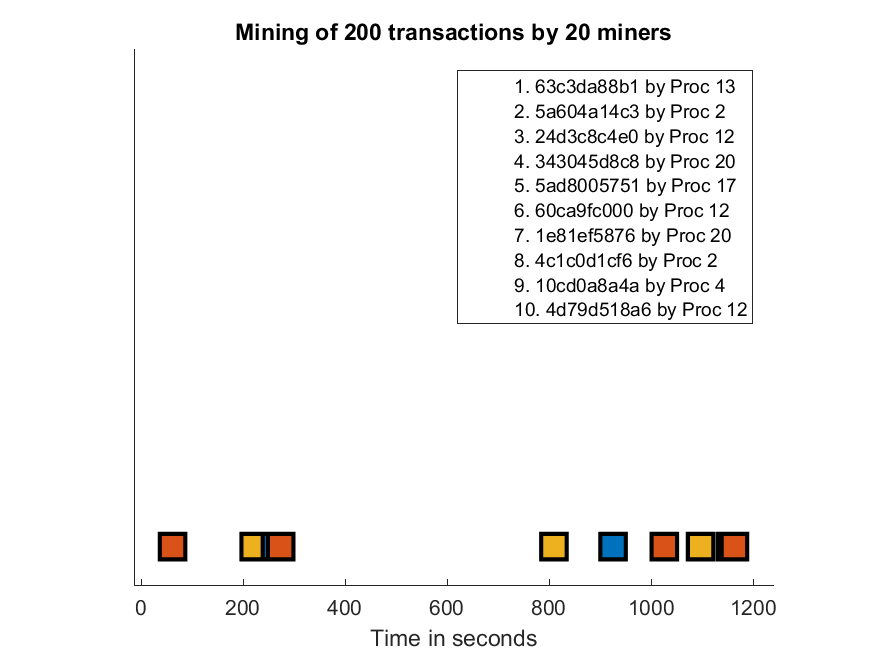
\includegraphics[width=10cm]{Figures/timeline_1}
\caption{Timeline for the 10 first blocks}
\end{figure}
\medskip


\section{Can we improve our model?} \label{improvements}

Here are some ideas to improve our simulation: \newline

\begin{itemize}
  \item The possibility to choose the network structure. To do so, we could use an adjacency matrix: \newline

  \begin{figure}[ht]
  \centering
  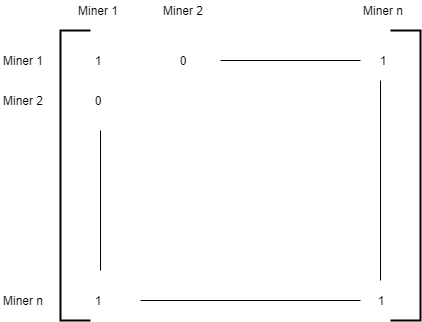
\includegraphics[width=8cm]{Figures/matrix}
  \caption{Example of an adjacency matrix}
  \end{figure}
  \medskip

  An adjacency matrix is symmetrical and 1 in the position (i, j) indicates that the miner i and j are neighbors. For example, in the figure above, the miner 1 and n are neighbors but not the miner 1 and 2. \newline

  With this method, we could try several network structures and analyze their influence on the mining process.

  \item The possibility to create pools. We could create a function which defines if a miner belongs to a pool or not: \newline

  \[
    isInPool(miner) =
    \begin{cases}
      0, & \text{if the miner doesn't belong to a pool}  \\
      i > 0, & \text{if the miner belongs to the pool i} \\
    \end{cases}
  \]
  \medskip

  Then, when a miner successfully mined a block, we share the reward with the pool if he belongs to one. With the method, we could try to implement the 51\% attack.

  \item Implementing the selfish mining attack. We've implemented the finite state machine which models this attack but we could also try to implement this algorithm for real to observe the results match.


\end{itemize}
